
\begin{figure}[h!]

  \centering    
    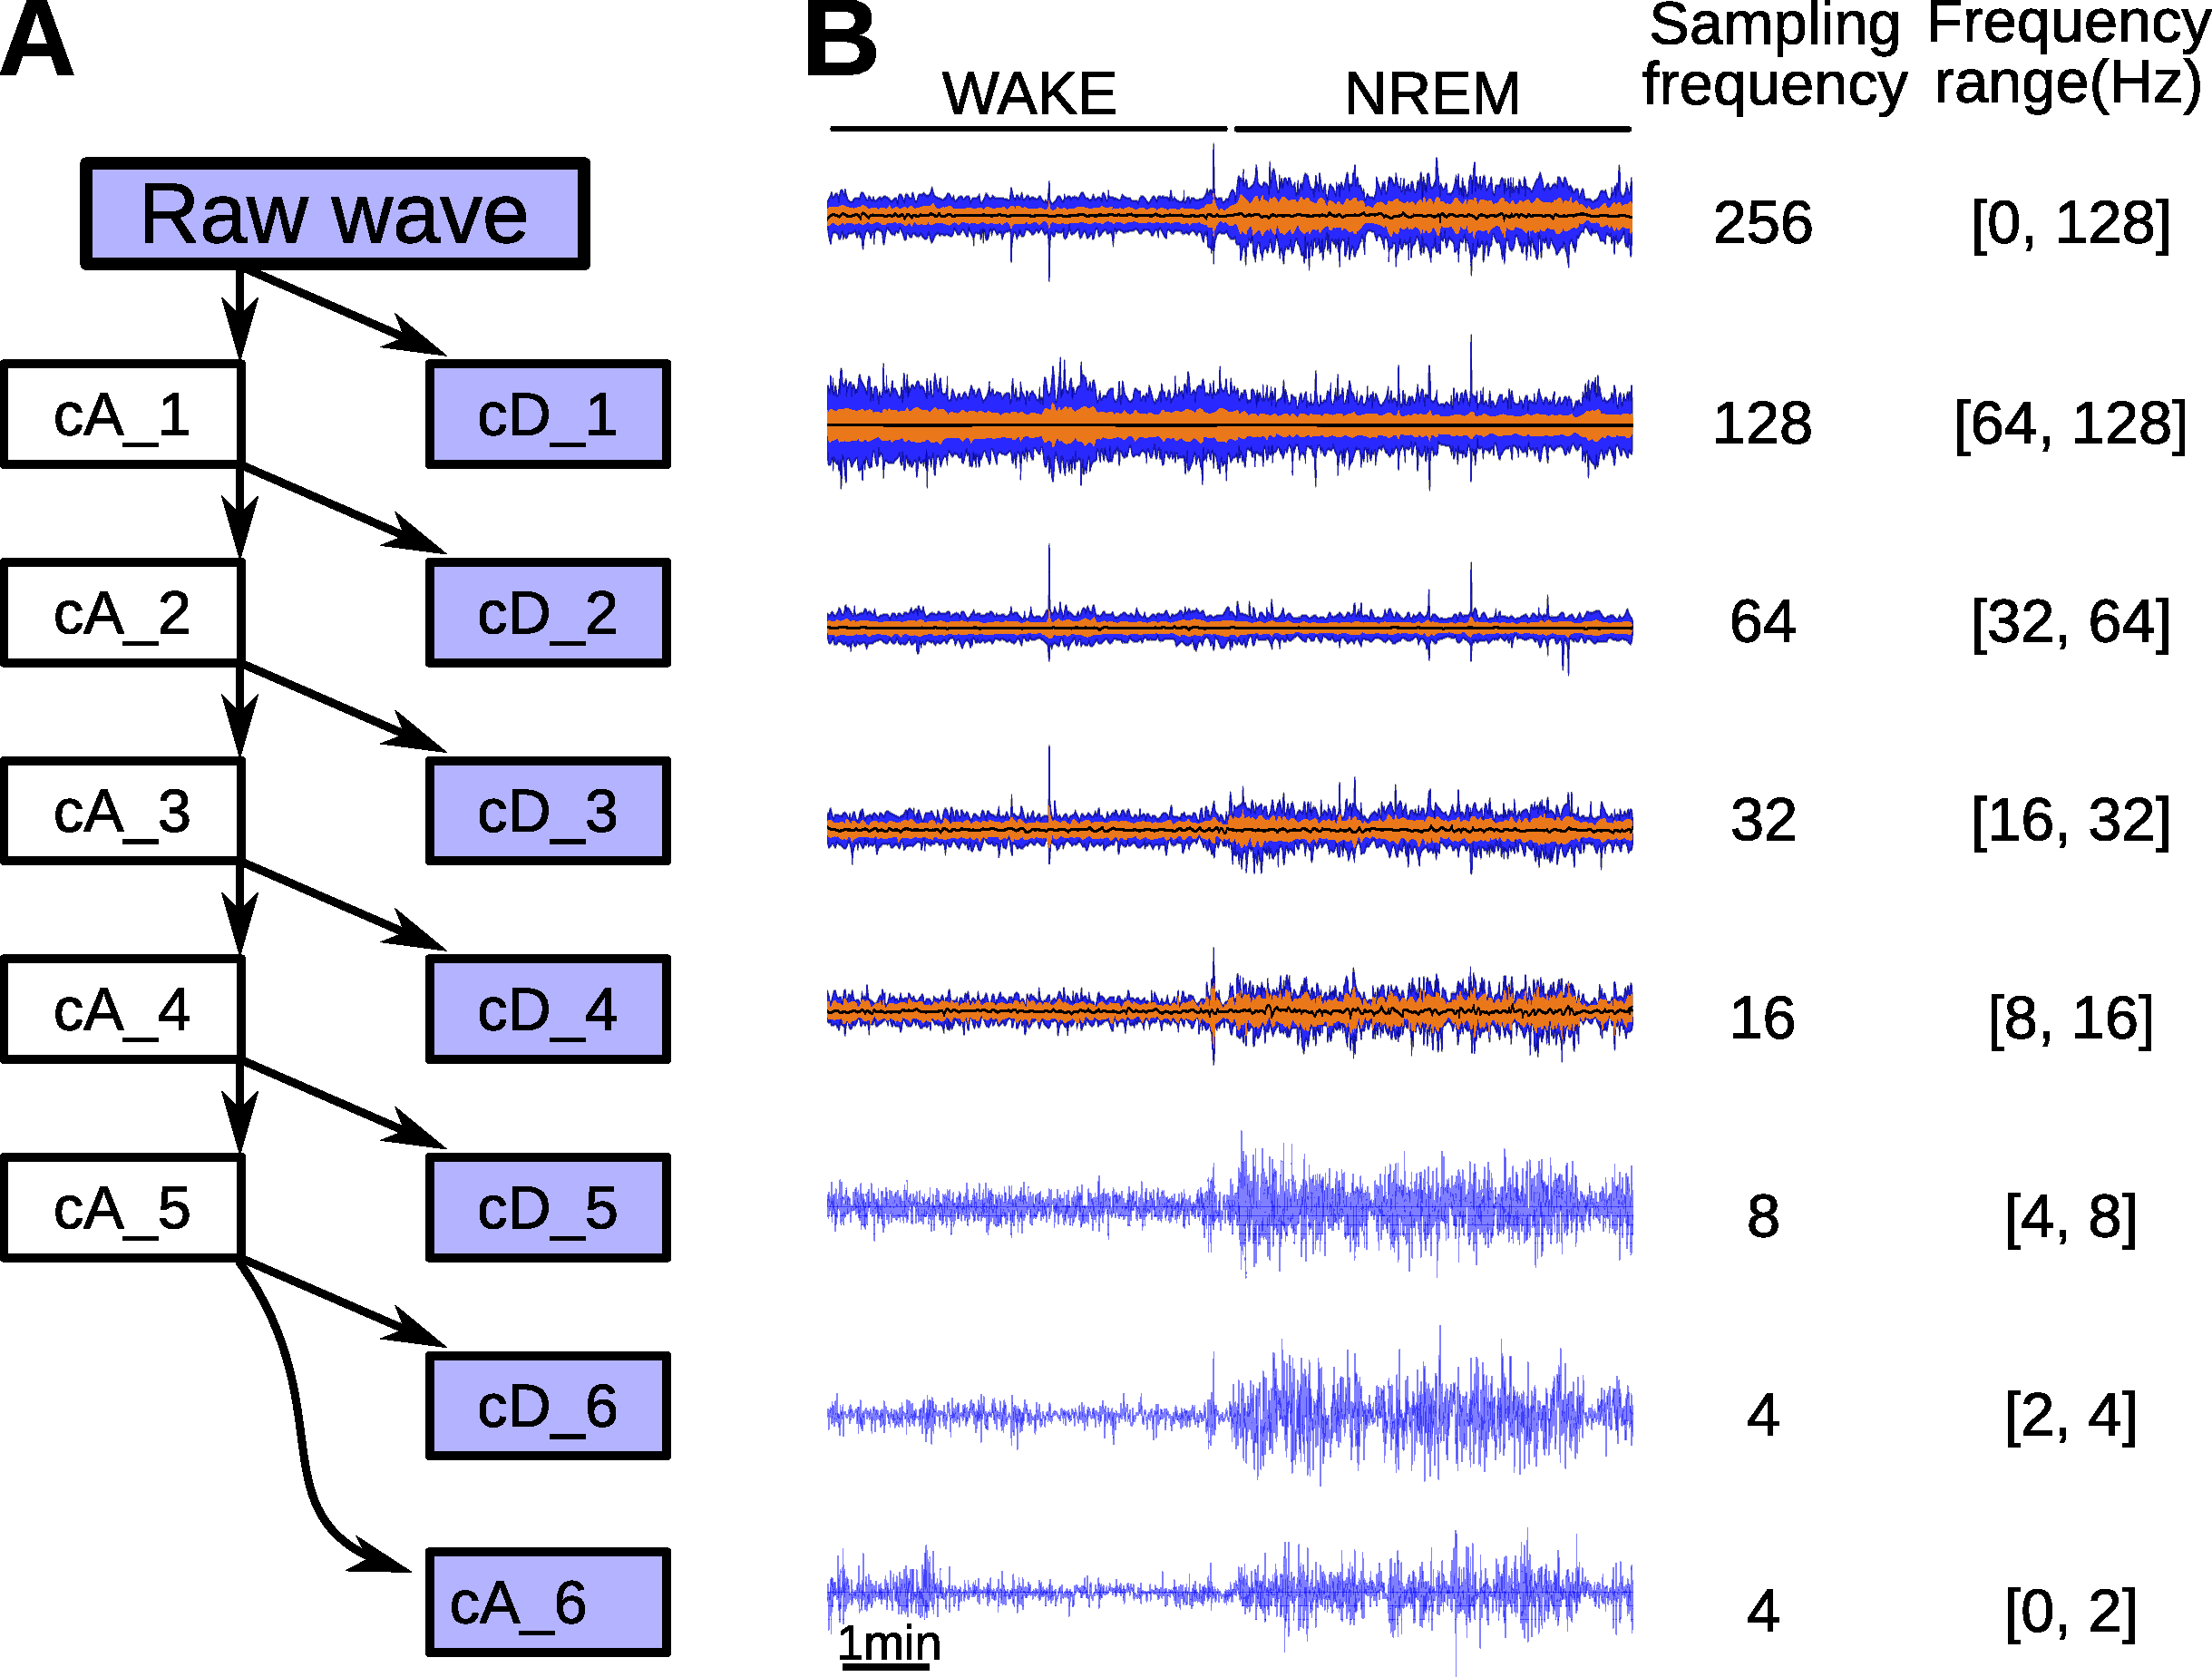
\includegraphics[width=0.95\textwidth]{figures/dwd.pdf}
  \caption{\ctit{Discrete waveletet decomposition.}
  The initial signal is split into pairs of coefficients: A and D. They capture the low ($[0, f_s/2]$), and high $[f_s/2, f_s]$ frequency information, respectively.
  Discrete wavelet transform is applied iteratively on subsequent A coefficients. In this example, decomposition is performed up to the sixth level.
  Ten minutes representing the \gls{eeg} of a transition between a wake and a slow wave sleep(NREM) are shown for the raw wave and each of the coefficients that are kept for feature extraction(blue rectangles). 
  Later, each of the eigth time series is segmented into five second epochs, and features are exhaustively computed for all wavelet coefficients as well as the raw signal.
  In this figure, the five first signals are too dense to be displayed in a naive fashion. Instead, only local range(blue), inter-quantile range (orange) and median (black line) are represented.
  \label{fig:dwd}
  }
           
\end{figure}

